\subsection{Méthode directe}
Les méthodes de résolution directe permettent de résoudre exactement l'équation $Ax=b$.
%
Parmi ces méthodes, la décomposition LU est la plus utilisée.
%
La factorisation LU correspond à la factorisation d'une matrice $A$ en deux matrices triangulaires $L$ et $U$ tel que $L.U=A$ (Fig.~\ref{fig:lu_3}).
%
Grâce à cette factorisation, résoudre l'équation $Ax=b$ est équivalent à résoudre successivement les équations $Ly=b$ et $Ux=y$.
%
Ces deux équations peuvent être résolues facilement parce que les matrices $L$ et $U$ sont triangulaires (Algo.~\ref{algo:trsv}).

%   (-_-)   %
\begin{figure}[!h]
  \centering
  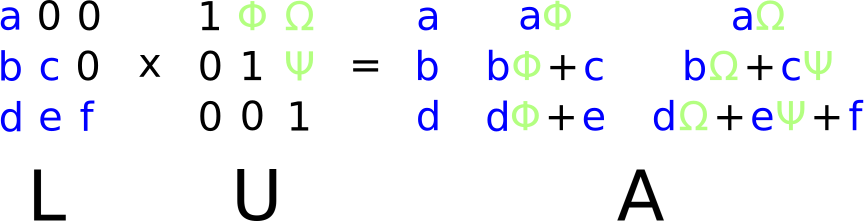
\includegraphics[width=\textwidth]{lu_3}
  \caption{Exemple d'égalité entre une matrice $A$ et le produit de deux matrices triangulaire $L$ et $U$}
  \label{fig:lu_3}
\end{figure}

\begin{algorithm}
  \KwData{$L$ : Matrice triangulaire inférieure\\
    $U$ : Matrice triangulaire supérieure\\
    $x$ : Vecteur des inconnues\\
    $y$ : Vecteur temporaire\\
    $b$ : Vecteur donné\\
    $n$ : Taille des matrices}
  \For{$i=1$ {\bf à} $n$} {
    $sum := 0$\\
    \For{$j=1$ {\bf à} $i-1$} {
      $sum += L_{ij} * y_j$ \\
    }
    $y_i := (b_i-sum)/L_{ii}$ \\
  }
  \For{$i=n$ {\bf à} $1$} {
    $sum := 0$\\
    \For{$j=n$ {\bf à} $i+1$} {
      $sum += U_{ij} * x_j$ \\
    }
    $x_i := (y_i-sum)/U_{ii}$ \\
  }
  \caption{Résolutions triangulaires}
  \label{algo:trsv}
\end{algorithm}

L'algorithme~\ref{algo:lu} représente la construction des matrices triangulaires $L$ et $U$ à partir de $A$.
%
Par contre, cet méthode présente un problème de remplissage.
%
Les matrices $L$ et $U$ contiennent beaucoup plus d'éléments non-nuls que la matrice $A$.
%
Cette augmentation du nombre d'éléments peut conduire à ne plus pouvoir stocker les matrices $L$ et $U$ à cause du manque d'espace mémoire.


\begin{algorithm}
  \KwData{$A$ : Matrice à factoriser \\
    $n$ : Taille de la matrice}
  \For{$i=1$ {\bf à} $n$} {
    \For{$j=1$ {\bf à} $i-1$} {
      \For{$k=j+1$ {\bf à} $n$} {
        $A_{ik} -= A_{ij}*A_{jk}$
      }
    }

    \For{$j=i+1$ {\bf à} $n$} {
      $A_{ij} /= A_{ii}$
    }
  }
  \caption{Factorisation LU sur place.}
  \label{algo:lu}
\end{algorithm}

%   (-_-)   %
\begin{figure}[!h]
  \centering
  \includegraphics[width=\textwidth]{lu_example}
  \caption{Exemple de factorisation LU d'une matrice creuse avec remplissage.}
  \label{fig:lu_example}
\end{figure}

Les méthodes directes ont l'avantage de fournir une solution exacte au problème $Ax=b$.
%
Par contre, ces méthodes sont coûteuse aussi bien en mémoire qu'en calcul.
%
Pour un cas 3D à $n$ inconnues, nous aurons un stockage en O($n^{3/2}$) et une complexité en nombre d'opérations en O($n^2$).
%
En simulation de réservoir, la valeur $n$ peut être grande (supérieur à 1~000~000).
%
Il n'est donc pas envisageable d'utiliser ce genre de méthode.
